% Sections about the game: history, how to play, the numbered HUD, scoring and lives, tips.
\sect{5. The original game}

\textbf{Commando} (\textit{Senj\=o no \=Okami}, ``Wolf of the Battlefield'', in Japan) was released by Capcom for arcades
in May 1985. It was designed by Tokuro Fujiwara, who was making \textit{Ghosts'n Goblins} at the same time. You are
\textbf{Super Joe}, a soldier dropped by helicopter alone in enemy territory, who must fight his way out on foot, armed with a
rifle and a few grenades.

It was one of the most successful arcade games of 1985 in the USA and the UK, and its home versions topped the charts
that Christmas. It made the vertical run-and-gun game popular, and had many imitators such as SNK's \textit{Ikari Warriors}.
Its sequel was \textit{Mercs} (1989), and Super Joe came back in \textit{Bionic Commando}. This version keeps the arcade
game as it was: its eight areas, its enemies, its music and its rules.

\sect{6. How to play}

You walk up the screen through the enemy lines. Soldiers come from every side, run at you and shoot; others wait in
trenches, behind sandbags or in bunkers, and mortars, jeeps, trucks and motorcycles join them along the way.

\begin{itemize}
\item \textbf{You lose a life} if a bullet hits you, if a soldier or a vehicle reaches you, if an explosion (a grenade or a
mortar shell, including your own grenade) goes off next to you, or if you walk into the river.
\item \textbf{Grenades} are your weapon against what the rifle cannot hurt: bunkers, trucks, mortars and soldiers behind
cover. One grenade can take out several enemies at once, and that is worth a bonus.
\item \textbf{Prisoners.} Now and then a prisoner is led across the screen by guards. Shoot all the guards and the prisoner
is free.
\item \textbf{Grenade boxes} lie on the ground: walk over one to pick up 1, 3 or 5 grenades.
\item \textbf{Officers.} Now and then a soldier in green runs across the screen without shooting: an officer running away.
Shoot him for 2000 points.
\item \textbf{End of an area.} At the end of each area the screen stops in front of a gate. Soldiers pour out of it; when
they have all come out and been defeated, Super Joe walks through the gate and a short picture closes the area.
\item \textbf{Areas.} There are four areas in a round; the fourth ends at a fortress, where the helicopter picks you up and
flies you to the next round (areas 5 to 8). After area~8 the game starts over from area~1, and it goes on until you lose your
last life. Each area cleared adds a medal to the panel.
\end{itemize}

\begin{figure}[H]
\centering
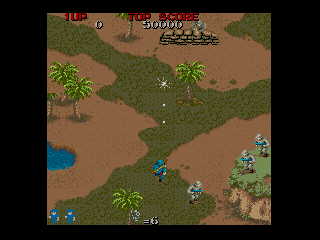
\includegraphics[width=0.48\textwidth]{../img/manual-area1.png}\hfill
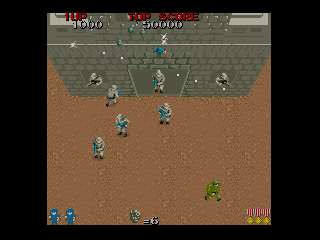
\includegraphics[width=0.48\textwidth]{../img/manual-fortress.png}
\caption{Left: area 1, with a trench of sandbags. Right: the fortress at the end of area 4, with its soldiers coming out and
an officer in green running away.}
\end{figure}

\clearpage   % the panel heading stays with its picture
\sect{7. The status panel (HUD)}

The score is at the top of the screen; your lives, grenades and medals at the bottom.

\begin{figure}[H]
\centering
\includegraphics[width=0.46\textwidth]{img/hud.png}
\caption{The game screen and its status panel.}
\end{figure}

\begin{tabularx}{\textwidth}{@{}cp{3.6cm}X@{}}
\toprule
\textbf{\tNo} & \textbf{\tElement} & \textbf{\tTellsYou}\\
\midrule
1 & \texttt{1UP} & Your score.\\
2 & \texttt{TOP SCORE} & The best score of the ranking (50000 at power-on).\\
3 & Lives & The lives you have left, apart from the one you are playing.\\
4 & Grenades & The grenades you have left.\\
5 & Medals & One medal for every area you have cleared.\\
\bottomrule
\end{tabularx}

\sect{8. Score, lives and records}

\begin{itemize}
\item \textbf{Lives.} You start with 3. You get an extra life at \textbf{10,000} points and then every \textbf{50,000} points.
\item \textbf{After losing a life} you start again from the last point you passed, with at least 6 grenades. The game also
starts with 6 grenades; you can carry up to 99.
\item \begin{minipage}[t]{\linewidth}\textbf{Points.}
\begin{center}
\begin{tabular}{@{}lr@{}}
\toprule
Soldier & 200 to 500\\
Soldier behind cover & 200\\
Officer in green & 2000\\
Guard of a prisoner & 1000\\
Prisoner freed & 1000\\
Mortar & 500\\
Bunker (two grenades) & 500 + 1000\\
Truck / truck with gunner (grenade) & 500 / 1000\\
Jeep (seven shots) & 200 per shot\\
Grenade box & 1000\\
Several enemies with one grenade (bonus) & 200 to 3000\\
Area cleared & 5000\\
\bottomrule
\end{tabular}
\end{center}\end{minipage}
\item \textbf{Records.} If your final score is among the best seven, you write your name: walk the soldier at the bottom
left and right to choose a column, move the cursor up and down to choose a row, and fire at a letter to write it. The dot and the
heart are letters too; the small \texttt{RB} sign erases the last letter and \texttt{ED} finishes. You have 60 seconds (\texttt{TIMER}).
The ranking is kept until the MSX is switched off.
\end{itemize}

\sect{9. Tips}

\begin{itemize}
\item Keep moving: most soldiers aim at where you are standing.
\item Save grenades for bunkers, mortars and trucks, and for the gate at the end of each area, where many soldiers come out
together.
\item A grenade that catches several soldiers is worth up to 3000 points of bonus.
\item Do not let the officers in green get away: 2000 points each.
\item Free the prisoners: 1000 points for each guard and 1000 more for the prisoner.
\item Keep your distance from your own grenades and from the mortar shells: their explosion is deadly for you too.
\end{itemize}
